\documentclass{article}
\usepackage{graphicx} % Required for inserting images
\usepackage[polish]{babel}
\usepackage{hyperref}
\usepackage[T1]{fontenc}
\usepackage{float}
\usepackage{listings}

\title{Dokumentacja - Winda}
\author{Filip Jędrzejewski}
\date{2 Czerwca 2024}

\begin{document}

\maketitle

\section{Opis modelowanego systemu}

Winda to system transportu pionowego, który głównie umożliwia przemieszczanie się osób między różnymi poziomami budynku. Działanie windy opiera się na kilku kluczowych elementach:

\begin{enumerate}
    \item \textbf{Panel przycisków:} Pasażerowie wybierają piętro docelowe, naciskając odpowiedni przycisk na panelu (w windzie lub poza nią - przyciski na poszczególnych piętrach).
    \item \textbf{Sterowanie:} Sygnały z przycisków są przekazywane do sterownika windy, który analizuje żądania i podejmuje decyzje dotyczące ruchu kabiny.
    \item \textbf{Silnik:} Silnik elektryczny porusza kabiną windy w odpowiednim kierunku.
    \item \textbf{Kabina:} Kabina windy porusza się w szybie windowym przewożąc pasażerów.
    \item \textbf{Drzwi:} Drzwi kabiny i drzwi zewnętrzne (piętra) otwierają się i zamykają automatycznie, umożliwiając bezpieczne wejście i wyjście pasażerów.
    \item \textbf{Wyświetlacz:} Wyświetlacz informuje pasażerów o aktualnym położeniu kabiny.
\end{enumerate}

Cykl działania przykładowej windy:

\begin{enumerate}
    \item Pasażer naciska przycisk, wskazując piętro docelowe.
    \item Sterownik windy odbiera sygnał i analizuje go, uwzględniając aktualne położenie kabiny i inne żądania.
    \item Sterownik wysyła polecenie do silnika, aby rozpocząć ruch w odpowiednim kierunku.
    \item Silnik napędza kabinę poruszającą się w szybie windowym.
    \item Gdy kabina osiągnie żądane piętro, sterownik wysyła polecenie do silnika, aby zatrzymać windę.
    \item Sterownik wysyła polecenie do drzwi kabiny i drzwi piętra, aby się otworzyły.
    \item Pasażerowie wchodzą lub wychodzą z windy.
    \item Po określonym czasie lub po naciśnięciu przycisku zamknięcia drzwi, sterownik wysyła polecenie zamknięcia drzwi.
    \item Po zamknięciu drzwi, winda jest gotowa do przyjęcia kolejnego żądania (cykl się powtarza).
\end{enumerate}


\section{Spis komponentów}

\subsection{Komponenty typu \texttt{data}}

\subsubsection{ElevatorState}

Kod:

    \begin{lstlisting}[basicstyle=\ttfamily, keywordstyle=\bfseries]
data ElevatorState
    properties
        Data_Model::Enumerators => ("Idle", "MovingUp", "MovingDown",
                                     "DoorOpening", "DoorClosing");
        Data_Model::Data_Representation => Integer;
        Data_Size => 4 Bytes;
end ElevatorState;

data implementation ElevatorState.impl
end ElevatorState.impl;
    \end{lstlisting}

    \texttt{ElevatorState} to enumerator, który reprezentuje możliwe stany windy. Komponent ten jest używany do śledzenia aktualnego stanu windy w systemie. W podanym modelu zdefiniowano pięć stanów:

    \begin{itemize}
        \item \textbf{Idle:} winda jest bezczynna, nie porusza się i ma zamknięte drzwi.
        \item \textbf{MovingUp:} Winda porusza się w górę.
        \item \textbf{MovingDown:} Winda porusza się w dół.
        \item \textbf{DoorOpening:} Drzwi windy są otwierane.
        \item \textbf{DoorClosing:} Drzwi windy są zamykane.
    \end{itemize}



    \subsubsection{ElevatorAction}

Kod:

    \begin{lstlisting}[basicstyle=\ttfamily, keywordstyle=\bfseries]
data ElevatorAction
end ElevatorAction;

data implementation ElevatorAction.impl
    subcomponents
        targetFloor: data FloorNumber;
        direction: data MotorCommand;
end ElevatorAction.impl;
    \end{lstlisting}

    \texttt{ElevatorAction} jest typem danych służącym do przekazywania informacji o żądanej akcji windy. W implementacji \texttt{ElevatorAction.impl}, widzimy, że składa się z dwóch subkomponentów:

    \begin{itemize}
        \item \textbf{targetFloor:} Określa piętro docelowe, na które winda ma się udać.
        \item \textbf{direction:} Określa kierunek ruchu windy
    \end{itemize}


    \subsubsection{FloorNumber}

    Kod:
    
        \begin{lstlisting}[basicstyle=\ttfamily, keywordstyle=\bfseries]
data FloorNumber
    properties
        Data_Model::Data_Representation => Integer;
        Data_Size => 4 Bytes;
end FloorNumber;

data implementation FloorNumber.impl
end FloorNumber.impl;
        \end{lstlisting}
    
        \texttt{FloorNumber} to typ danych reprezentujący numer piętra w budynku. W kontekście windy, \texttt{FloorNumber} jest używany do określania piętra docelowego, aktualnego piętra windy oraz do wyświetlania informacji o piętrze na panelu sterowania i wyświetlaczu w kabinie.
    

    \subsubsection{ButtonType}

    Kod:
    
    \begin{lstlisting}[basicstyle=\ttfamily, keywordstyle=\bfseries]
data ButtonType
    properties
        Data_Model::Enumerators => ("CallUp", "CallDown", "Cabin");
        Data_Model::Data_Representation => Integer;
        Data_Size => 4 Bytes;
end ButtonType;

data implementation ButtonType.impl
end ButtonType.impl;
    \end{lstlisting}

    \texttt{ButtonType} to enumerator definiujący rodzaje przycisków obecnych w systemie windy. Ten typ danych jest używany w połączeniu z typem \texttt{FloorNumber} w strukturze \texttt{ButtonPress}, aby jednoznacznie określić, który przycisk został naciśnięty i na którym piętrze. Zawiera trzy wartości:

    \begin{itemize}
        \item \textbf{CallUp:} Przycisk wywołania windy na wyższe piętro, umieszczony na zewnątrz kabiny.
        \item \textbf{CallDown:} Przycisk wywołania windy na niższe piętro, umieszczony na zewnątrz kabiny.
        \item \textbf{Floor:} Przycisk wyboru konkretnego piętra, znajdujący się wewnątrz kabiny windy.
    \end{itemize}


    \subsubsection{ButtonPress}

    Kod:
    
    \begin{lstlisting}[basicstyle=\ttfamily, keywordstyle=\bfseries]
data ButtonPress
    properties
        Data_Size => 8 Bytes; 
end ButtonPress;

data implementation ButtonPress.impl
    subcomponents
        floor: data FloorNumber;
        button_type: data ButtonType;
end ButtonPress.impl;
    \end{lstlisting}

    \texttt{ButtonPress} to struktura reprezentująca zdarzenie naciśnięcia przycisku w windzie. Zawiera ona dwa elementy:

    \begin{itemize}
        \item \textbf{floor:} Przechowuje numer piętra, na którym przycisk został naciśnięty (lub na jakie ma się udać).
        \item \textbf{button\_type:} Określa rodzaj naciśniętego przycisku (góra, dół lub piętro).
    \end{itemize}

    Te informacje są kluczowe dla systemu sterowania windą, ponieważ umożliwiają mu określenie, na które piętro winda powinna się udać i w jakim kierunku.



    
    \subsubsection{MotorCommand}

    Kod:
    
    \begin{lstlisting}[basicstyle=\ttfamily, keywordstyle=\bfseries]
data MotorCommand
    properties
        Data_Model::Enumerators => ("Up", "Down", "Stop");
        Data_Model::Data_Representation => Integer;
        Data_Size => 4 Bytes;
end MotorCommand;

data implementation MotorCommand.impl
end MotorCommand.impl;
    \end{lstlisting}

    \texttt{MotorCommand} to enumerator definiujący możliwe polecenia sterujące dla silnika windy. Kontroler silnika interpretuje to polecenie i steruje silnikiem windy zgodnie z nim. Zawiera trzy wartości:

    \begin{itemize}
        \item \textbf{Up:} Polecenie ruchu windy w górę.
        \item \textbf{Down:} Polecenie ruchu windy w dół.
        \item \textbf{Stop:} Polecenie zatrzymania windy
    \end{itemize}


    \subsubsection{DoorCommand}

    Kod:
    
    \begin{lstlisting}[basicstyle=\ttfamily, keywordstyle=\bfseries]
data DoorCommand
    properties
        Data_Model::Enumerators => ("Open", "Close");
        Data_Model::Data_Representation => Integer;
        Data_Size => 4 Bytes;
end DoorCommand;

data implementation DoorCommand.impl
end DoorCommand.impl;
    \end{lstlisting}

    \texttt{DoorCommand} to enumerator określający możliwe polecenia dla drzwi windy. Zawiera dwie wartości:

    \begin{itemize}
        \item \textbf{Open:} Polecenie otwarcia drzwi windy.
        \item \textbf{Close:} Polecenie zamknięcia drzwi windy.
    \end{itemize}



    \subsubsection{DoorState}

    Kod:
    
    \begin{lstlisting}[basicstyle=\ttfamily, keywordstyle=\bfseries]
data DoorState
    properties
        Data_Model::Enumerators => ("Opened", "Closed", "Opening", "Closing");
        Data_Model::Data_Representation => Integer;
        Data_Size => 4 Bytes;
end DoorState;

data implementation DoorState.impl
end DoorState.impl;
    \end{lstlisting}

    \texttt{DoorState} to enumerator reprezentujący możliwe stany drzwi windy. Zawiera on cztery wartości:

    \begin{itemize}
        \item \textbf{Opened:} Drzwi są całkowicie otwarte.
        \item \textbf{Closed:} Drzwi są całkowicie zamknięte.
        \item \textbf{Opening:} Drzwi są w trakcie otwierania.
        \item \textbf{Closing:} Drzwi są w trakcie zamykania.
    \end{itemize}



    \subsection{Komponenty typu \texttt{thread}}

    
    \subsubsection{ButtonPanelThread}

    Kod:
    
    \begin{lstlisting}[basicstyle=\ttfamily, keywordstyle=\bfseries]
thread ButtonPanelThread
    features
        button_press_in: in event data port ButtonPress;
        button_data_out: out data port ButtonPress;
    properties
        SEI::MIPSBudget => 15.0 mips;
end ButtonPanelThread;

thread implementation ButtonPanelThread.impl
end ButtonPanelThread.impl;
    \end{lstlisting}

    \texttt{ButtonPanelThread} jest wątkiem odpowiedzialnym za obsługę panelu przycisków w windzie. Jego głównym zadaniem jest odczytywanie sygnałów z przycisków i przekazywanie informacji o naciśnięciach do \texttt{ButtonPanelController}. Wątek \texttt{ButtonPanelThread} jest kluczowym elementem systemu windy, ponieważ umożliwia pasażerom komunikowanie swoich żądań do systemu.

    


    
        








\subsection{Schemat rozwiązania}

W celu rozwiązania zadania stworzono następujący diagram \texttt{Orange}:


\begin{figure}[H]
    \centering
    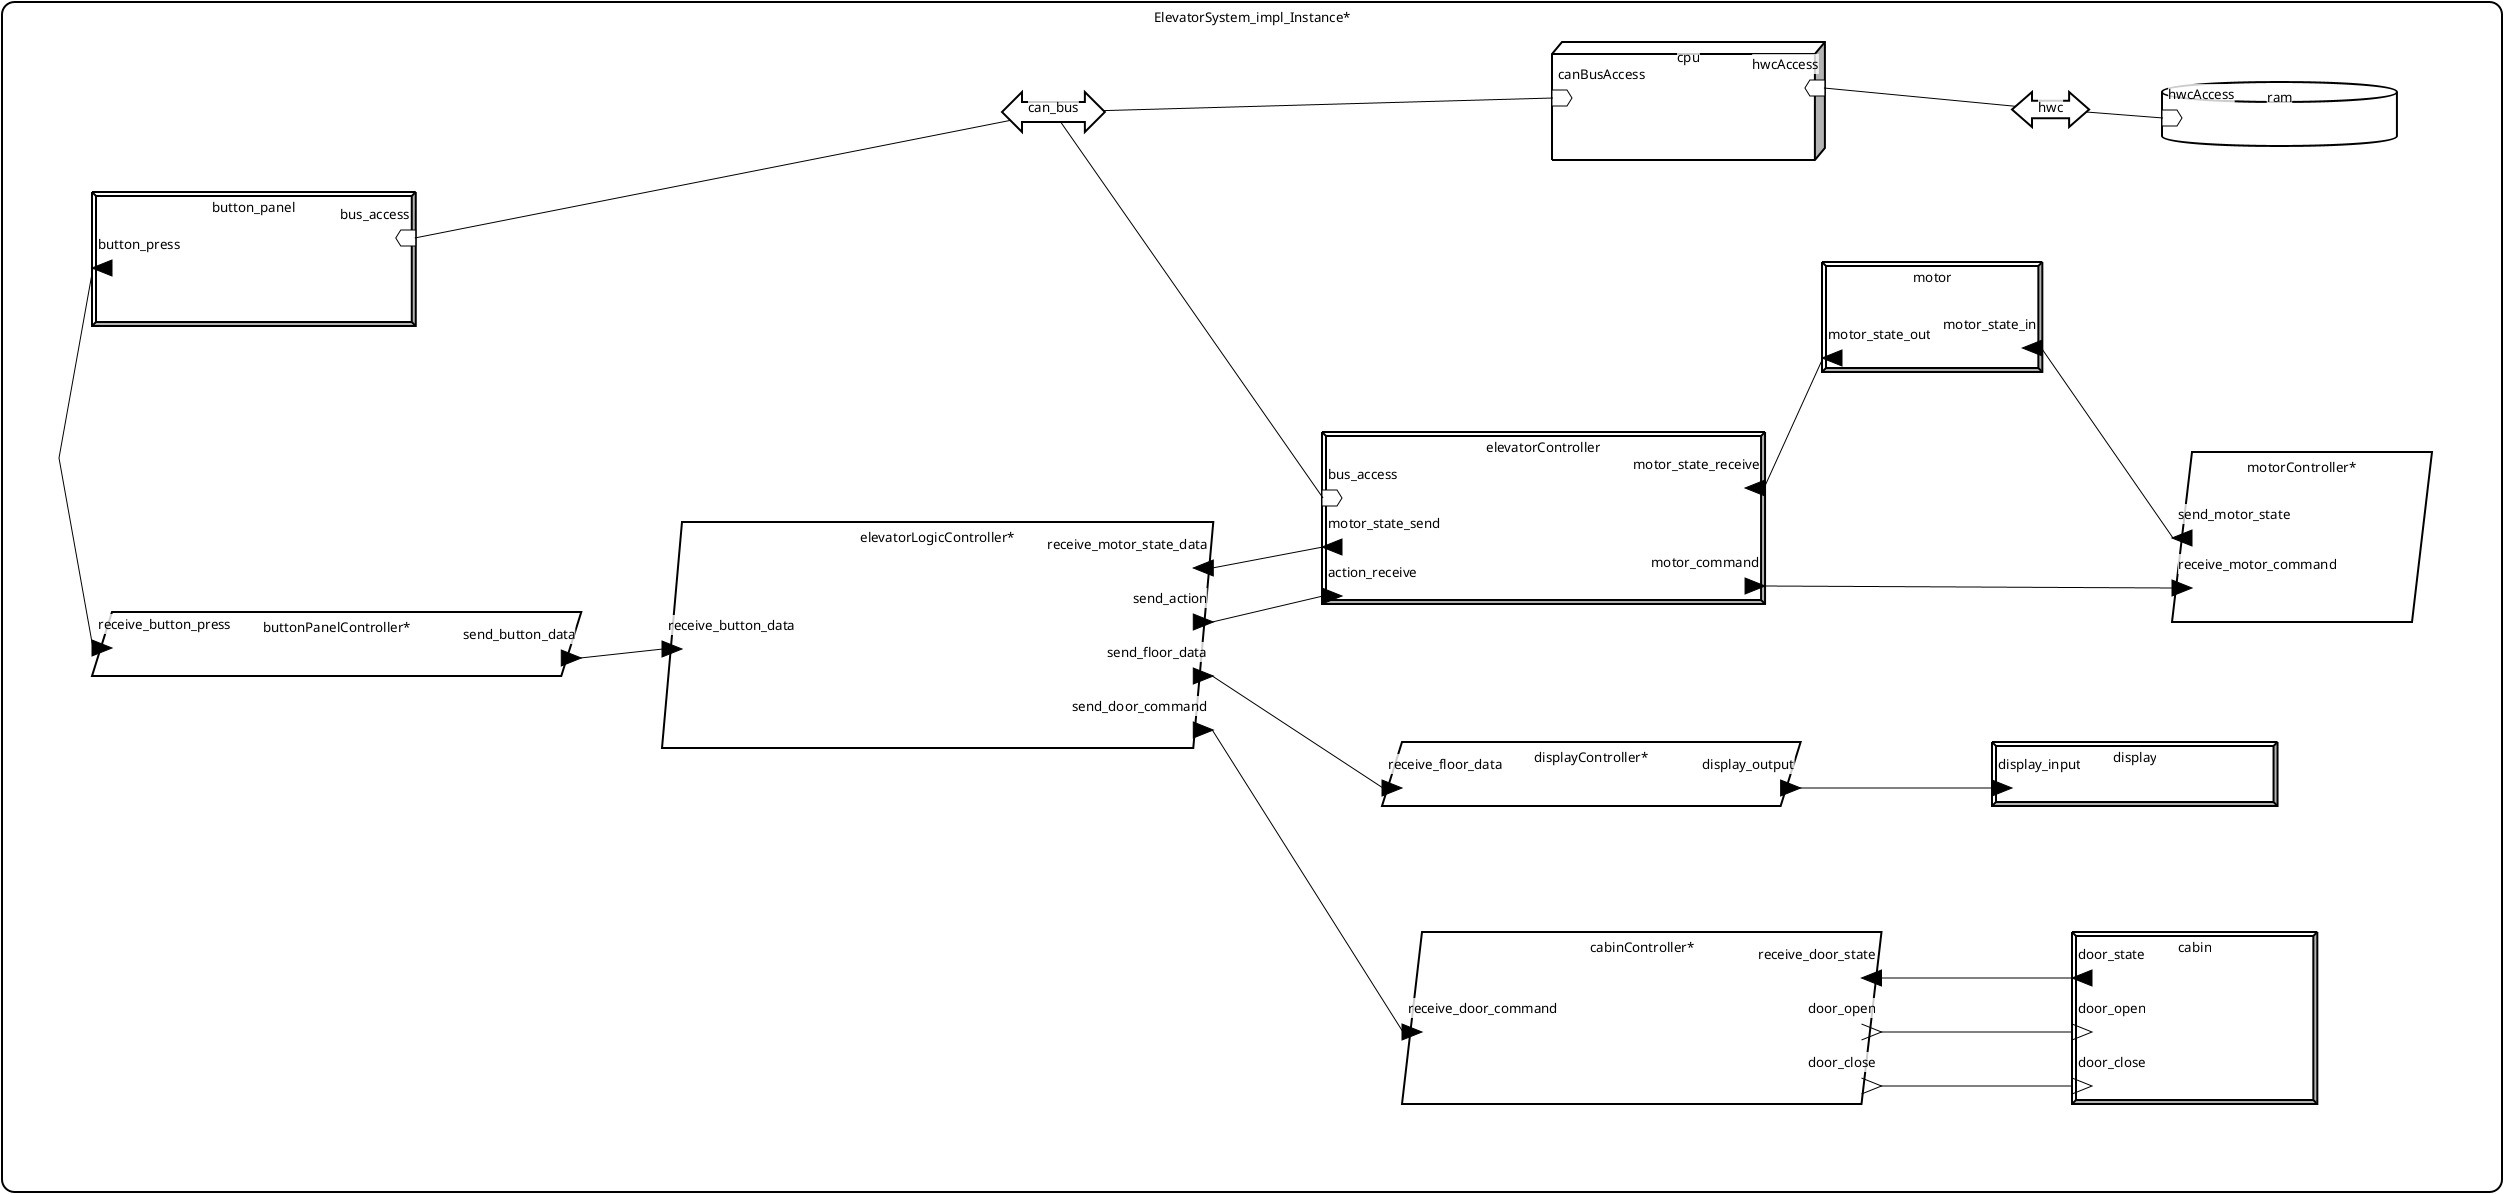
\includegraphics[width=1.2\linewidth]{./images/schema.png}
\end{figure}













\end{document}